\documentclass[12pt,a4paper]{article}
\usepackage[margin=25mm]{geometry}
\usepackage[utf8]{inputenc}
\usepackage[magyar]{babel}
\usepackage{graphicx}
\usepackage{t1enc}
\usepackage{float}
\selectlanguage{magyar}

\title{Boltie - Specifikáció \\[1ex] \large Mobilszoftver Laboratórium félévközi feladat}
\author{Wágner Árpád\\(O2OFFX)}
%\date{2022 Március}

% Szükséges árubeolvasási típusok:
%   - Betárazás
%   - Eladás
%   - Visszáru (Lehetne opcionális)
%   - Selejt
%
% Esetleg éttermeknek lehetne olyasmi, hogy Az asztalt is ki lehessen választani, pl speciális QR kóddal.
% Legyen olyan áru, aminek nincs darabszáma (pl helyben készült étel, kedvezmény, stb)
% Akciók kezelése! (Bár lehet, h ez inkább backend)

% BEJELENTKEZÉS: felhasználó azonosítás, majd egy speciális vonalkód beolvasása, amely az adott egységet azonosítja.


\begin{document}
	
	\pagenumbering{gobble}
	\maketitle
	\vfill
	\tableofcontents
	\vfill
	\newpage
	\pagenumbering{arabic}
	
	\section{A szoftver célja}
	A Boltie különböző boltok vagy vendéglátóipari egységek számára készülő szoftver, lényege, hogy az áruk kezelését és azok eladását segítse úgy, hogy képes azok raktározását illetve eladását kezelni a vonalkódjuk beolvasásának segítségével.
	
	A szoftver célközönsége elsősorban kis- és középvállalatokból tevődik össze, akik ezen szoftver használatával nagyobb beruházás nélkül is képesek lesznek az áruikat vagy szolgáltatásaikat hatékonyan kezelni.
	
	A Boltie a felhasználási területéből adódóan nem tartalmazhat reklámokat, ám elvárható, hogy a felhasználók a használatáért fizessenek (akár havi vagy éves előfizetési rendszerben is).
	
	\textit{\textbf{Megjegyzés:} ebben a dokumentumban több helyen használom a ``vonalkód'' szót. Fontos megjegyezni, hogy ez nem csak a hagyományos vonalkódod jelenti, hanem bármilyen egyéb hasonló funkcionalitású technológiát is (pl QR-kód stb).}
	
	\section{Felhasználói történetek}
	A felhasználói történetek az alábbi formában íródnak: \texttt{Mint \textit{felhasználótípus}; képes vagyok arra \textit{egy feladatot elvégezni}; hogy ennek segítségével \textit{elérjek egy célt}}. (Az egyes részegységek pontosvesszővel vannak elválasztva egymástól.)\newline
	Az alábbiakban olvashatók a felhasználói történetek felhasználótípus szerint csoportosítva.
	\subsection{Manager}
	\begin{itemize}
		\item Mint manager;\newline meg tudom tekinteni, hogy egy árusító helyen milyen a jelenlegi árukészlet;\newline hogy szükség szerint új árukat is tudjak rendelni.
		\item Mint manager;\newline el tudok végezni minden feladatot, amit az eladók is;\newline  hogy amennyiben szükséges, én is el tudjam látni ezeket a feladatokat is.
	\end{itemize}
	
	\subsection{Eladó}
	\begin{itemize}
		\item Mint eladó;\newline be tudom olvasni egy termék vonalkódját;\newline hogy azt eladjam.
		\item Mint eladó;\newline be tudok olvasni egy vonalkódot;\newline hogy azzal kedvezményt biztosítsak a vevőnek.
		\item Mint eladó;\newline be tudok olvasni egy vonalkódot;\newline hogy egy felhasználói csoportot beazonosítsak \textit{(pl egy asztalhoz számoljam el a következő termékeket)}.
		\item Mint eladó;\newline be tudok olvasni egy vonalkódot;\newline hogy sztornózzak egy terméket vagy vásárlást.
		\item Mint eladó;\newline el tudok végezni minden feladatot, amit az árufeltöltők is;\newline  hogy amennyiben szükséges, én is el tudjam látni ezeket a feladatokat is.
	\end{itemize}
	
	\subsection{Árufeltöltő}
	\begin{itemize}
		\item Mint árufeltöltő;\newline be tudom olvasni egy termék vonalkódját;\newline hogy azt betárazzam.
		\item Mint árufeltöltő;\newline be tudom olvasni egy termék vonalkódját;\newline hogy azt selejtként számoljam el.
		\item Mint árufeltöltő;\newline be tudom olvasni egy termék vonalkódját;\newline hogy azt visszáruként számoljam el.
	\end{itemize}
	
	\subsection{Minden felhasználó}
	Az itt leírtak minden felhasználótípusra vonatkoznak.
	\begin{itemize}
		\item Mint általános felhasználó;\newline azonosítani tudom magam;\newline hogy hozzáférjek az alkalmazás funkcióihoz.
		\item Mint általános felhasználó;\newline be tudok olvasni egy speciális vonalkódot;\newline hogy kiválaszthassam, épp melyik konkrét üzletben dolgozok.
	\end{itemize}
	
	\section{Használati esetek}
	Az előbbiekben a felhasználói történetekben leírt funkciókat az \ref{fig:usecase} ábra  foglalja össze.
	\begin{figure}[H]
		\centering
		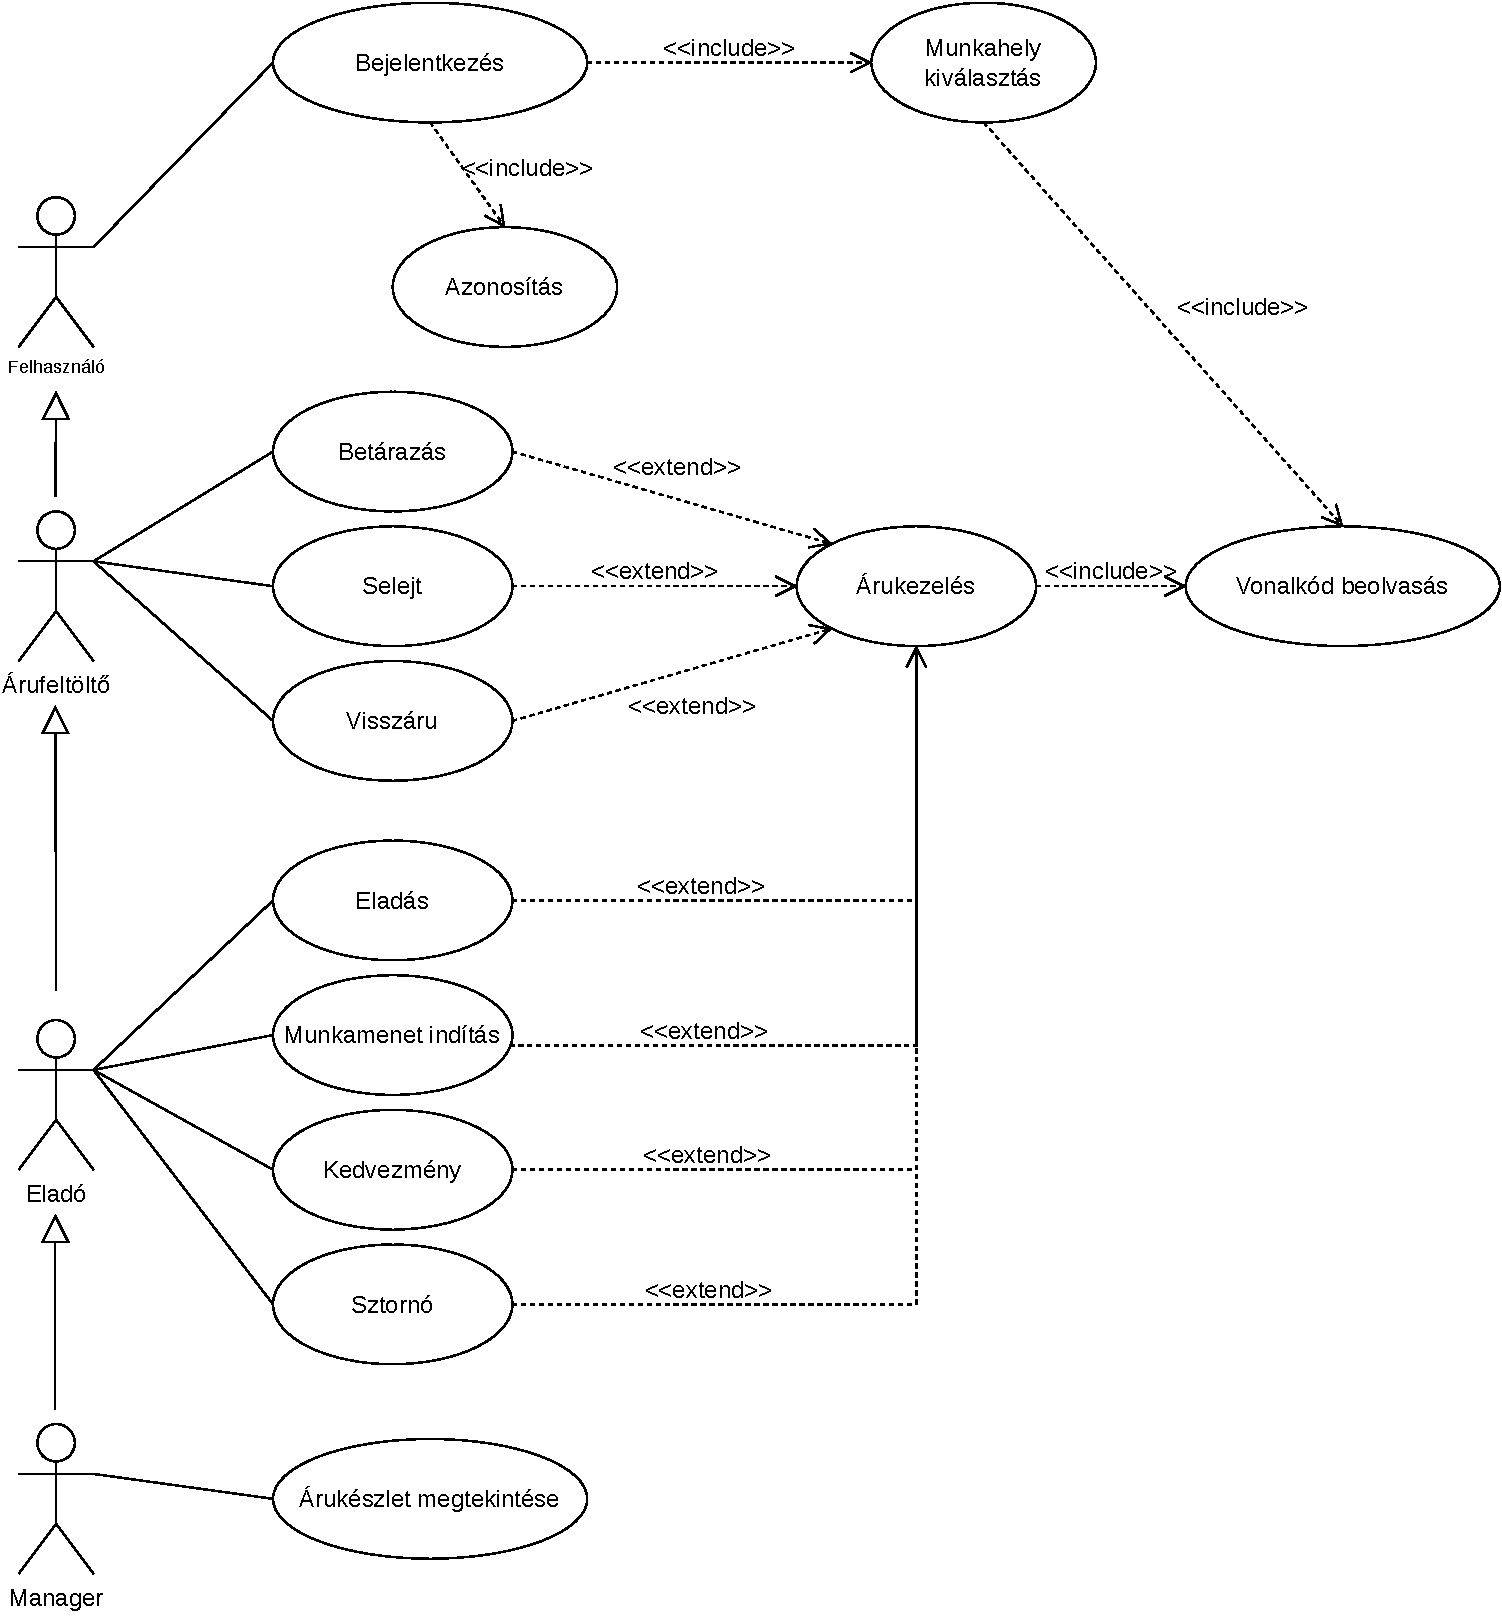
\includegraphics[width=0.9\textwidth]{img/usecases.pdf}
		\caption{A program használati esetei}
		\label{fig:usecase}
	\end{figure}
	
	\section{Felületterv}
	Az applikáció felhasználói felülete négy különböző képernyőből áll, melyek a következők:
	\begin{itemize}
		\item \textbf{Bejelentkezés:} Egyszerű bejelentkezési képernyő, mely emailt (vagy felhasználónevet), illetve egy jelszót vár.
		\item \textbf{Funkciókiválasztás:} Egy képernyőn láthatja a felhasználó a számára elérhető árukezelési funciókat és kiválaszthatja, hogy melyiket szeretné végezni.
		\item \textbf{Beolvasás:} A képernyő, amelyen a különböző típusú vonalkódok beolvasása történhet, adott esetben kiegészítő információkkal vagy interakciókkal.
		\item \textbf{Árulista:} Amennyiben a bejelentkezett felhasználó megfelelő jogosultságokkal rendelkezik, megtekintheti az aktuális árukészletet. Szükségesek különböző szűrők a jobb átláthatóság érdekében.
	\end{itemize}
	Ezek felületterve alább látható.
	\begin{figure}[H]
		\centering
		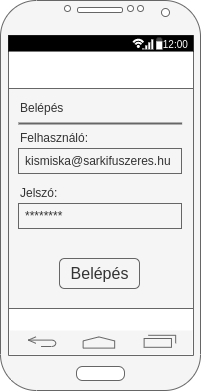
\includegraphics[width=0.5\textwidth]{img/login.png}
		\caption{A bejelentkezési képernyő}
		\label{fig:login}
	\end{figure}

	\begin{figure}[H]
		\centering
		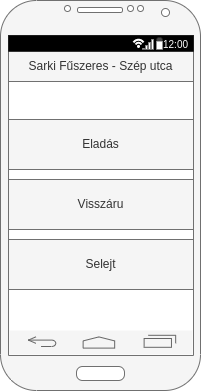
\includegraphics[width=0.5\textwidth]{img/functionselect.png}
		\caption{A funkcióválasztási képernyő}
		\label{fig:fnselect}
	\end{figure}
	
	\begin{figure}[H]
		\centering
		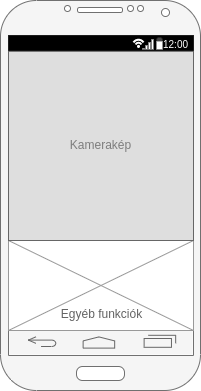
\includegraphics[width=0.5\textwidth]{img/scan.png}
		\caption{A beolvasási képernyő}
		\label{fig:scan}
	\end{figure}
	
\end{document}